
\chapter{Greifer Erkennung und Multi Task Lernen}
\label{chap:HauptteilMultiTaskLernen}
Als Kostenfaktor in DataScience-Projekten wurden die hohen Kosten zum Annotieren von Daten ermittelt. Im Autocrane-Projekt werden viele Aufgaben in einer Domäne durchgeführt. Als Frage stellt sich, ob eine geeignete Repräsentation der Domäne gefunden und ausgehend von dieser Repräsentation datensparsam (kostensparsam) aufgaben in dieser Domäne gelöst werden können.  


	\section{Greifererkennung auf Autoencoder}
	\label{sec:GreifererkennungAufAutoencoder}
    Autoencoder sind ein Ansatz um unüberwacht, also  ohne konkrete Aufgabe / Annotation, Repräsentationen zu finden. Ausgehend von dieser Repräsentation soll die  Aufgabe Greifererkennung gelöst werden. Hierzu wird auf die Datenrepäsentation des Autoencders eine Regression ausgeführt. In Abbildung \ref{ErgebnissRegressionAufAE} sind die Ergebnisse von drei Durchläufen abgebildet. Dieses Lösung erreicht deutlich schlechtere Ergebnisse als die Basislinie mit einer IoU von \todo{Iou Grapple}.
	\begin{figure}[h]
		\centering
		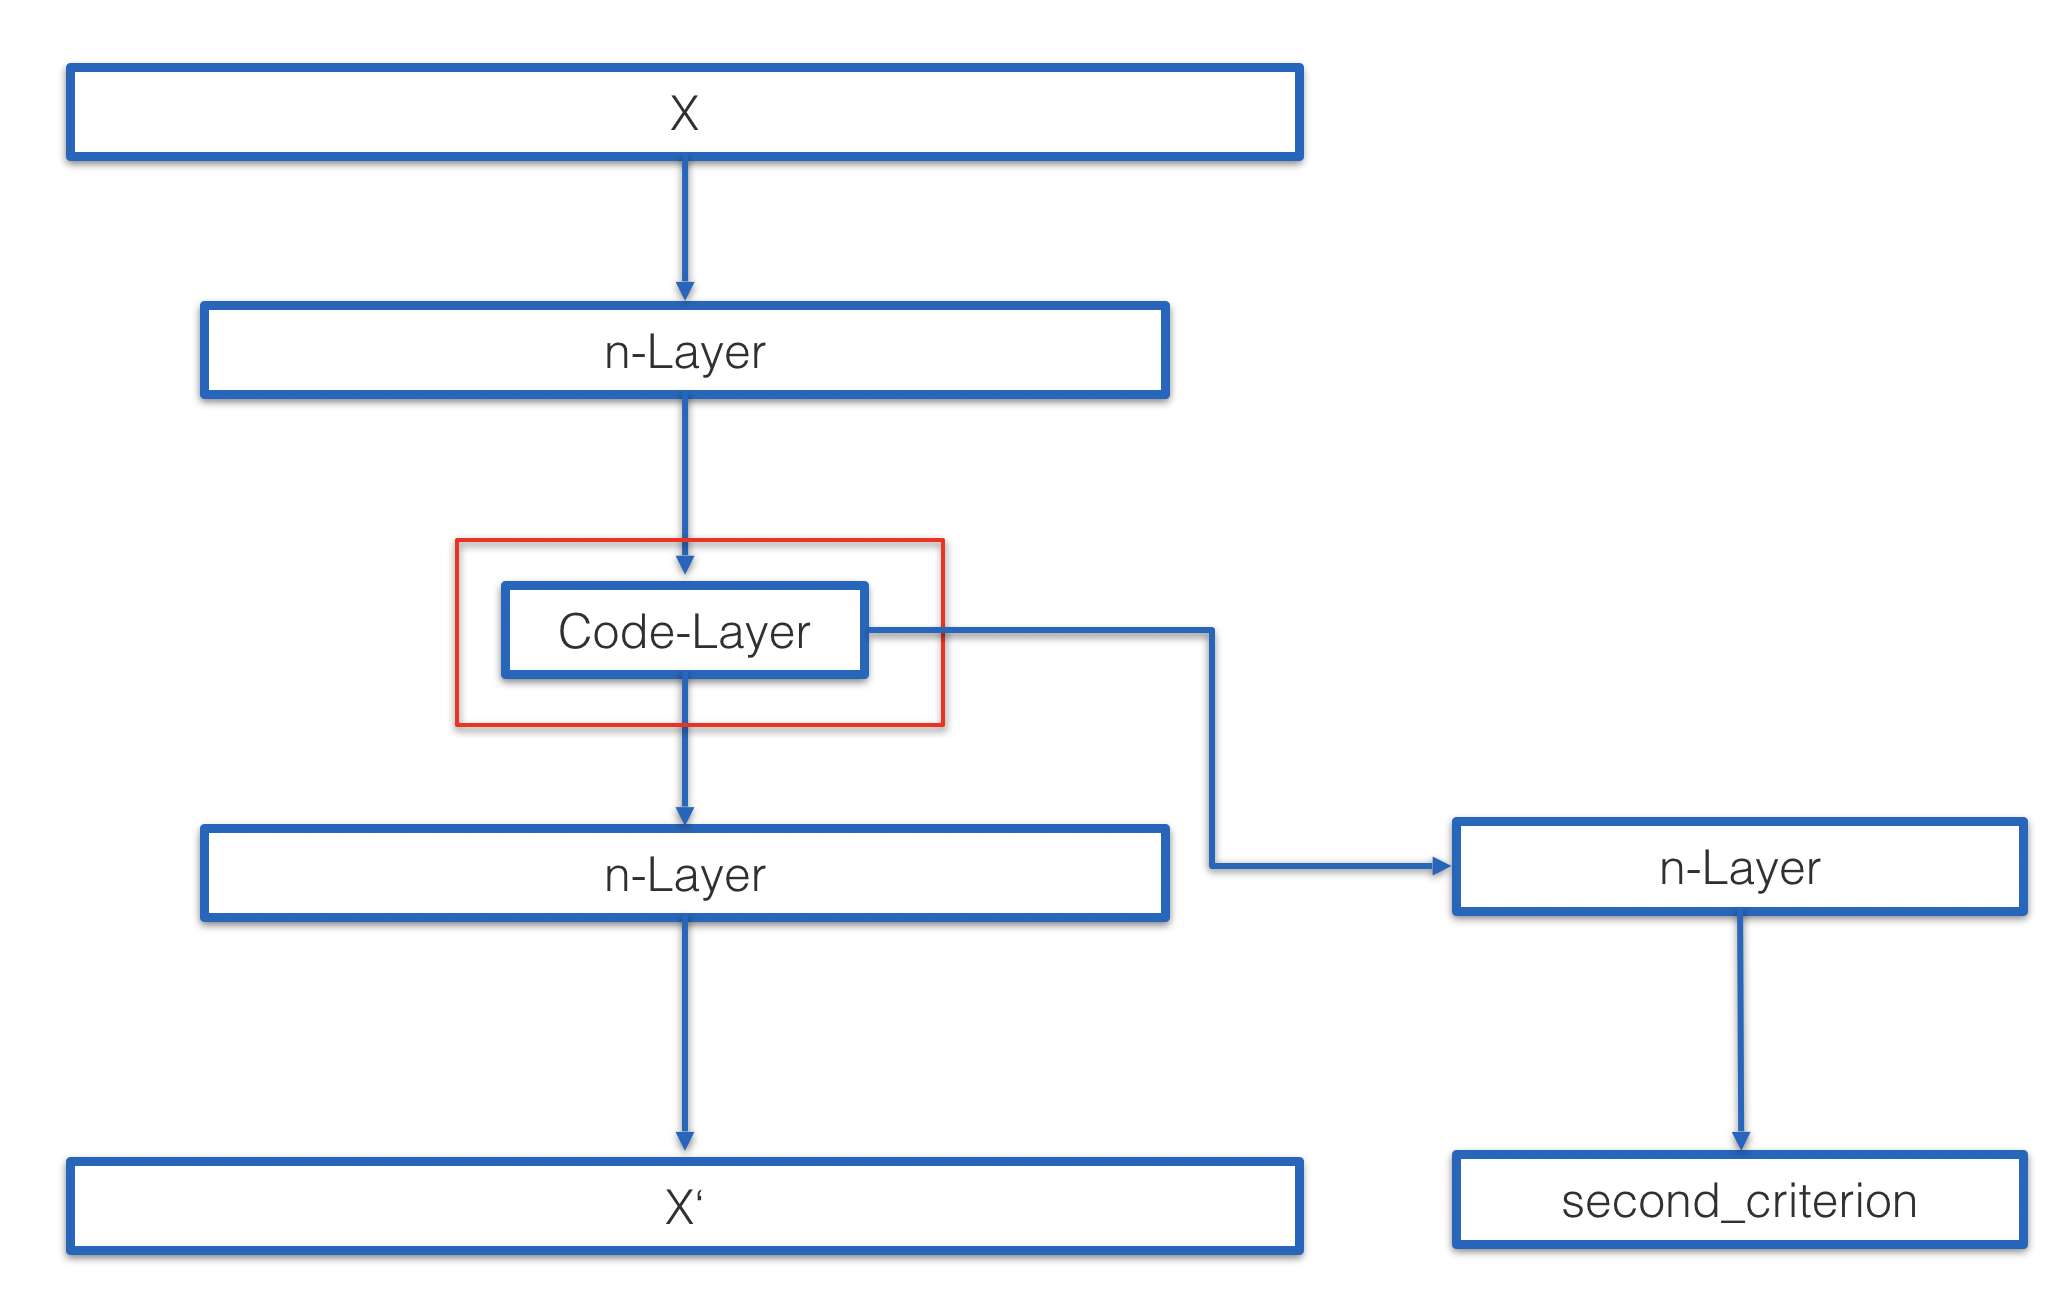
\includegraphics[width=0.5\textwidth, center]{bilder/Schema_Autoencoders/Schema_SCAE.png}
		\caption[Schema SecondCriterionAutoenocder]{Schema SecondCriterionAutoenocder}
		\label{img:ErgebnissRegressionAufAE}
	\end{figure}  
	In Abbildung \ref{todo Embedding} ist das Embedding des zugrundeliegenden Autoencoders abgebildet. Die Datenpunkte verteilen sich gut im Raum, bilden aber keine Merkmale des Greifers ab. In Abbildung \ref{todo Rekonstruktionen} sind Bilder mit ihren Rekonstruktionen abgebildet. Es ist sehr deutlich zu erkennen, dass sich der stark ändernde Hintergrund herausfordernd ist und in erster Linie die Lichtverhältnisse gelernt wurden.   
	
	\section{Mutli-Task Experiment}
	\label{sec:MultiTaskExperiment}
	Im Ansatz \ref{sec:GreifererkennungAufAutoencoder} wurde als schwäche des Ansatzes die fehlende Fokusierung des Autoencoders auf den Greifer ausgemacht. Multi-Task-Lernen soll durch gleichzeitiges bearbeiten der Aufgaben Repräsenation finden und Greifererkennung die schwäche des fehlenden Fokus kompensieren.   
	\subsection{Werkzeug}
	Zur Umsetzung der SIMO Multi-Task-Idee wurde ein Modul in Python erstellt. Das Werkzeug erweitert ... \todo{Werkezug beschreiben} 
	\subsection{Ergebnis}
	In Abbildung \ref{todo} bla blub
	
	In der Repräsentation werden die Merkmale des Greifers deutlich abgebildet. .....Vergleicht man die Rekosntruktionen des ersten Ansatzes mit denen des TaskFocusingAE lässt sich eine Fokusierung auf den Greifer erkennen. Besonders in Bild \ref{todo} zu sehen.
	
	\section{ConvolutionalSecondCriterionAutoenocder}
	\label{sec:SecondCriterionAutoenocder}
	Der SCAE erweitert einen ConvolutionalAutoencoder um ein weiteres Kriterium. Es gibt also zusätzlich zu der Rekonstruktion des Autoencoders einen weiteren Ausgang. Der zweite Ausgang kann wie jeder Ausgang für eine Binärklassifikation, für eine Multiklassifikation, für eine Regression oder jede andere beliebige Aufgabe genutzt werden. In Abbildung \ref{img:SchemaSCAE} ist der schematische Aufbau des SCAE abgebildet. Die Schichten des zweiten Kriteriums werden an die Code-Schicht des NN angehängt. Es können beliebig  viele Schichten genutzt werden. Die Verlustfunktion des NN besteht aus der Summe der einzelnen Verlustfunktionen und einer Gewichtung. Sie lautet im Detail: 
	\begin{align}
	loss = weight1 * loss\_autoencoder + weight2 * loss\_secondcriterion
	\end{align}
	Die Gewichtung der Verlustfunktionen kann dem SCAE per Konstruktor-Argument übergeben werden. Das Werkzeug ist als Python-Module implementiert. Dabei implementiert die Klasse ConvolutionalSecondCriterionAutoenocder den ConvolutionalAutoenocder aus Psipy. In Abbildung \ref{img:KlassendiagrammCSCAE} ist das Klassendiagramm des SCAE dargestellt.
	\begin{figure}[h]
		\centering
		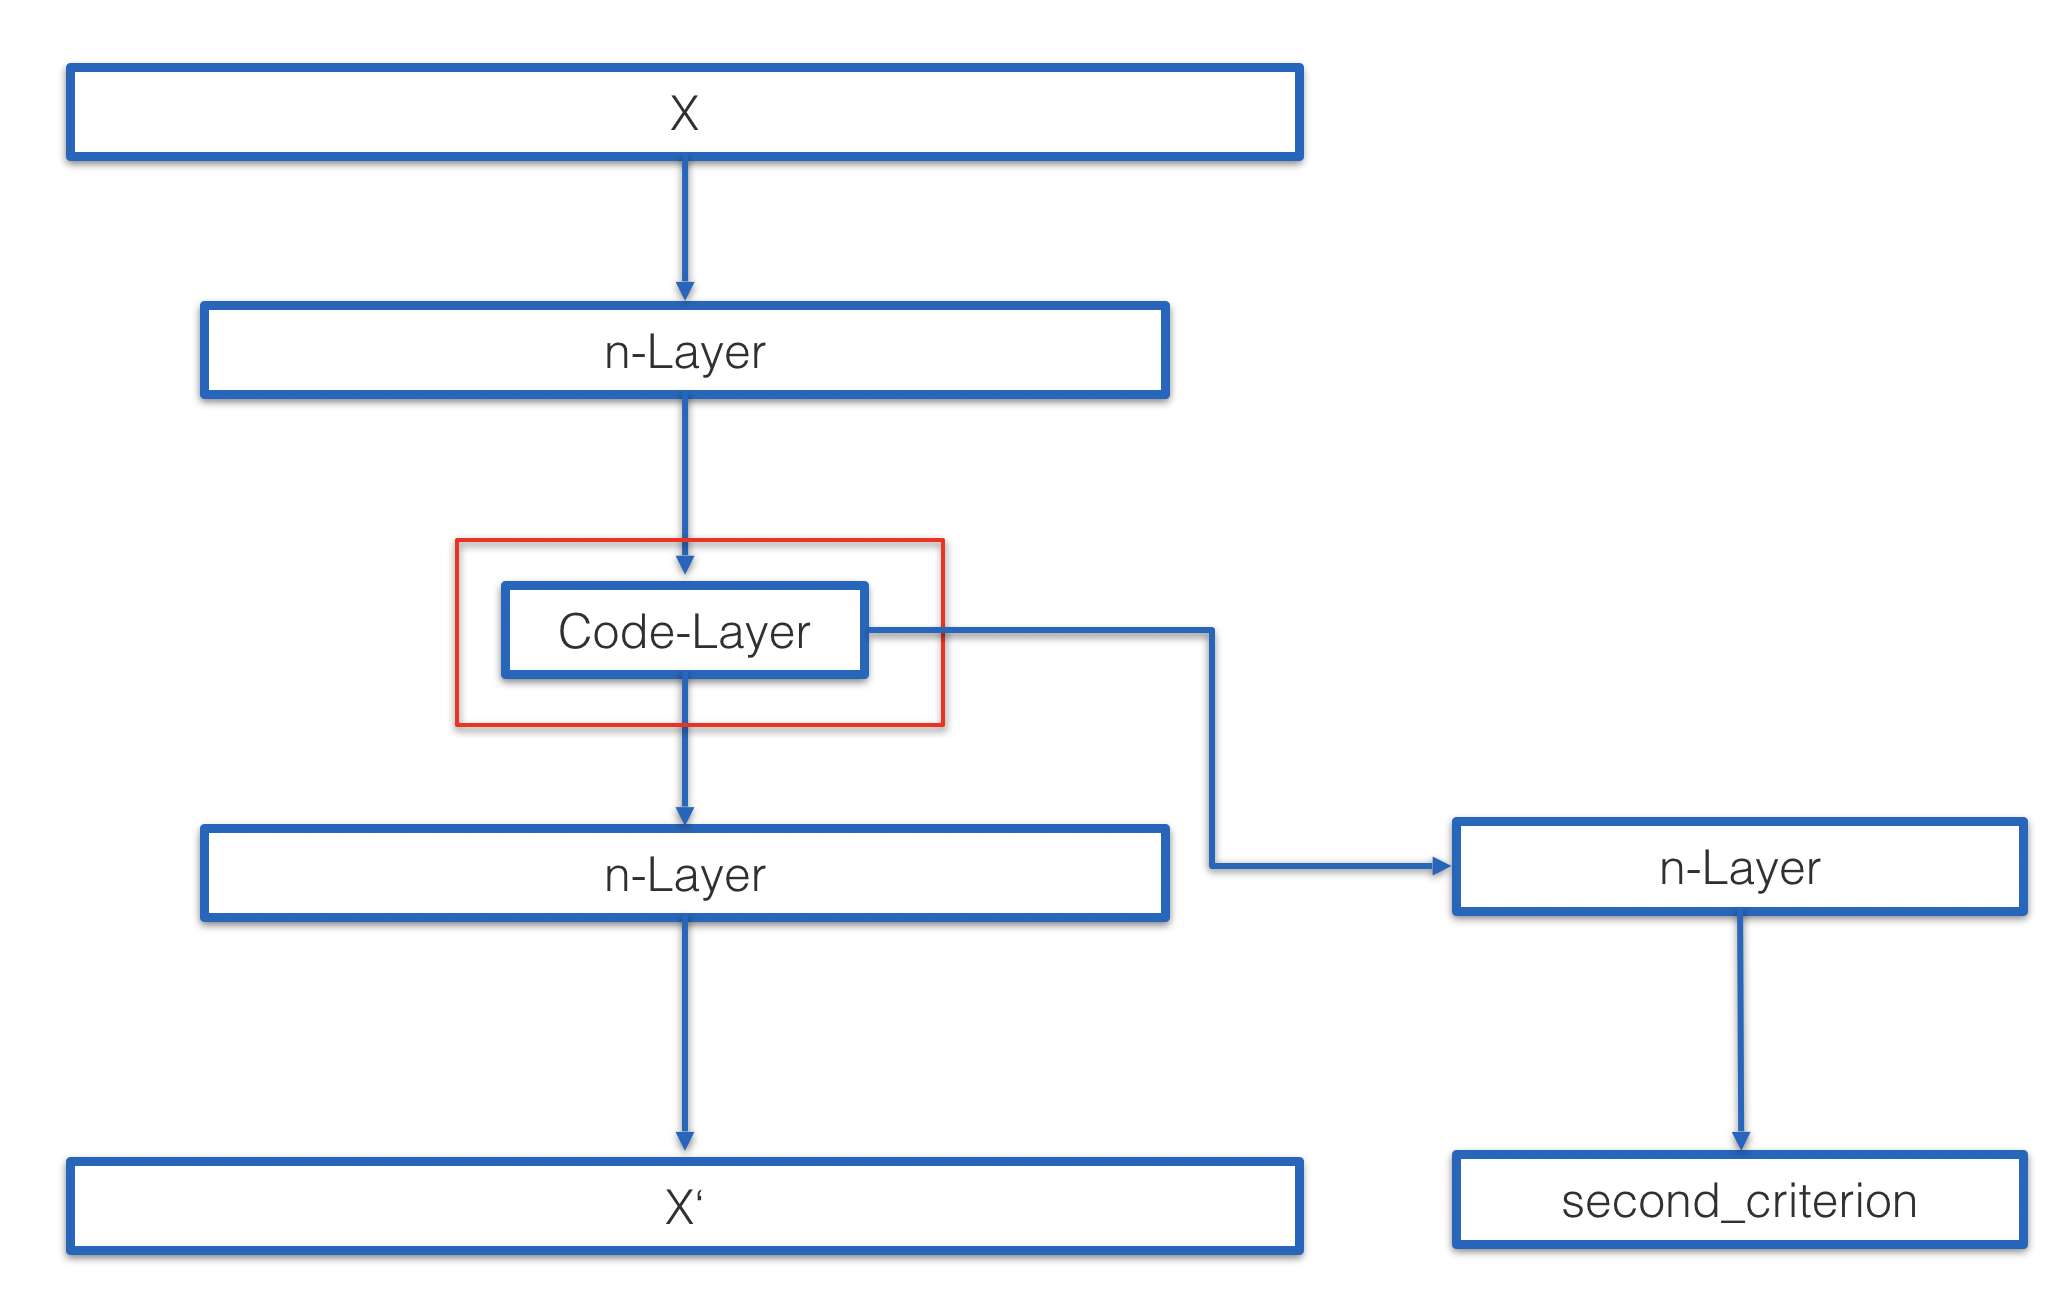
\includegraphics[width=0.5\textwidth, center]{bilder/Schema_Autoencoders/Schema_SCAE.png}
		\caption[Schema SecondCriterionAutoenocder]{Schema SecondCriterionAutoenocder}
		\label{img:SchemaSCAE}
	\end{figure}  
	\begin{figure}[h]
		\centering
		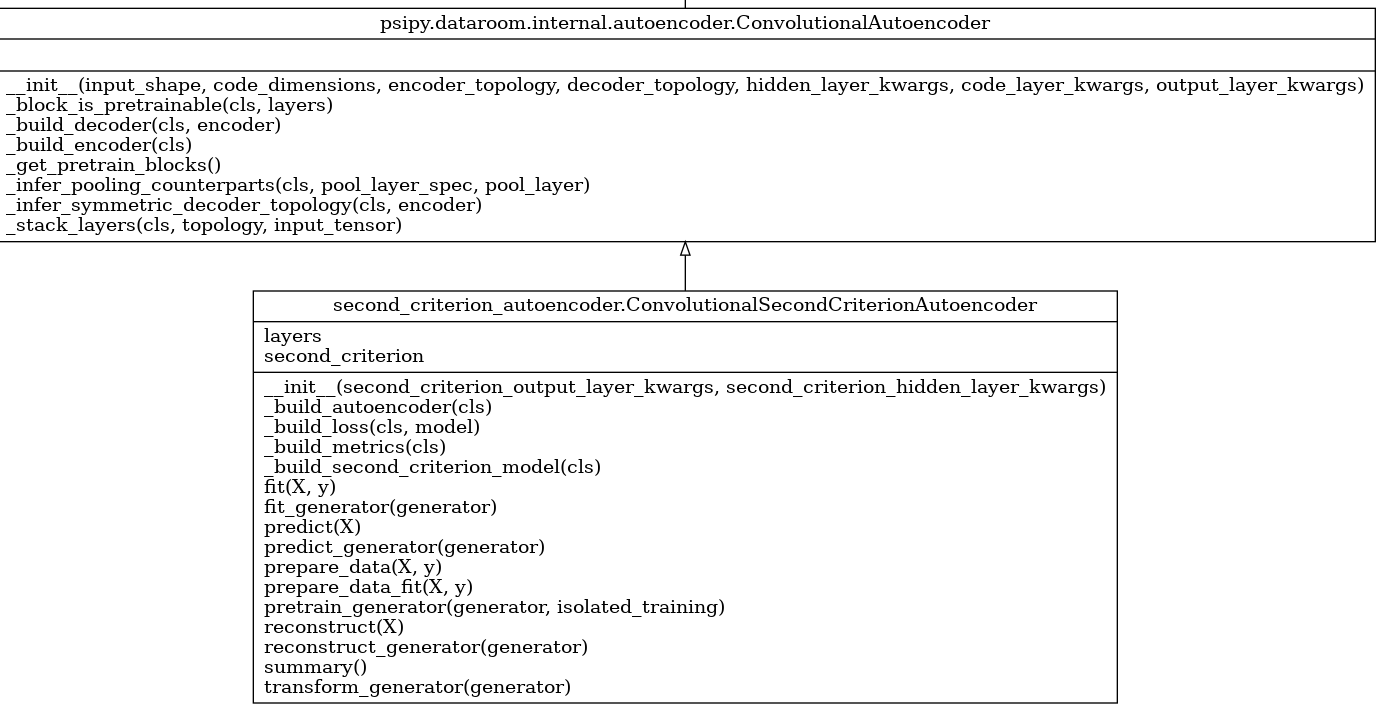
\includegraphics[width=0.5\textwidth, center]{bilder/Klassendiagramme/Klassendiagramm_CSCAE.png}
		\caption[Klassendiagramm ConvolutionalSecondCriterionAutoencoder]{Klassendiagramm ConvolutionalSecondCriterionAutoencoder}
	    \label{img:KlassendiagrammCSCAE}
	\end{figure}  
    Über den Konstruktor können alle Argumente welche zum Erstellen des Models notwendig sind per doppeltes Sternchen Wörterbuch Argument (**kwargs) an die Klasse übergeben werden. Diese Technik erlaubt es eine mit Schlüsselwörtern versehene Argumentliste variabler Länge zu übergeben. Die Argumentlisten werden beinahe in allen Methode zum Einsatz gebracht. Sie werden insbesondere genutzt, um Argumente an die zugehörigen Keras-Methoden zu übergeben. Die Namensgebung der Methode orientiert sich dabei an Keras. So wird z. B. in dem Methodenaufruf $fit(..)$ unter anderem auch die Keras-Methode  $fit(..)$ aufgerufen. Um einen SCAE zu trainieren, ist es notwendig eine Instanz zu erzeugen, die Methode $pretrain(..)$ aufzurufen und ihn anschließend mit der Methode $fit(..)$ zu trainieren.
    In dem Methodenaufruf $pretrain(..)$ wird das Modell erstellt und schichtenweise vortrainiert. Das eigentliche Training erfolgt in der Methode $fit(..)$. Alternativ können auch die zugehörigen Generatorenklassen aufgerufen werden.    
    
    In Listing \ref{lst:BspErstellungConvolutionalSecondCriterionAutoenocder} ist beispielhaft dargestellt, wie ein SCAE erstellt wird. In den ersten 10 Zeilen wird die Architektur erstellt. Ab Zeile 12 wird eine Instanz eines CSCA mittels Argumentenliste erstellt. Zu beachten ist, dass hier keine Decoder-Architektur übergeben wird. Wenn keine Decoder-Architektur bereitgestellt wird sie beim Erstellen des eigentlichen Modells aus der Encoder-Architektur abgeleitet.
	\begin{lstlisting}[language=python,caption=Beispiel Erstellung ConvolutionalSecondCriterionAutoenocder in Python, label=lst:BspErstellungConvolutionalSecondCriterionAutoenocder]
	encoder_topology = [("Conv2D", {"filters": 8, "kernel_size": (3, 3)}),
	("Conv2D", {"filters": 8, "kernel_size": (3, 3)}),
	('MaxPooling2D', {"pool_size": (2, 2)}),
	("Conv2D", {"filters": 16, "kernel_size": (3, 3)}),
	("MaxPooling2D", {"pool_size": (2, 2)}),
	("Conv2D", {"filters": 16, "kernel_size": (3, 3)}),
	("Flatten", {}),
	("Dense", {"units": 16})]

	second_criterion_topology = [("Dense", {"units": num_classes}) ]

	csca = ConvolutionalSecondCriterionAutoencoder(
	input_shape=(28, 28, 1),	
	code_dimensions=3, 
	encoder_topology=encoder_topology,
	second_criterion_topology=second_criterion_topology,
	hidden_layer_kwargs = {'activation': 'relu'},
	output_layer_kwargs = {'activation': 'sigmoid'},
	second_criterion_hidden_layer_kwargs = {'activation': 'relu'},
	second_criterion_output_layer_kwargs = {'activation': 'softmax'},
	second_criterion_loss = 'categorical_crossentropy',
	loss_weights=[8., 1.],
	second_criterion_metrics = {'second_criterion':'accuracy'},
	code_layer_kwargs=dict())
	\end{lstlisting}
Listing  \ref{lst:BspPretrainConvolutionalSecondCriterionAutoenocder}  zeigt den Aufruf der Methode Pretrain. Der Aufruf führt zu einem Schichtenweise-Trainieren des Netzwerkes mit den Daten x\_train bei 20 Epochen und einer Stapelgröße von 64. 
\begin{lstlisting}[language=python,caption=Beispielaufruf Pretrain  in Python, label=lst:BspPretrainConvolutionalSecondCriterionAutoenocder]
csca.pretrain(x_train,epochs = 20, batch_size = 64)
\end{lstlisting}

Der Methodenaufruf $fit(..)$ funktioniert wie der $fit(..)$-Aufruf in Keras. In Zeile drei des Listing  \ref{lst:BspPretrainConvolutionalSecondCriterionAutoenocder}  ist zu erkennen, dass die Zielgrößen der verschiedenen Ausgänge einfach als Python-Wörterbuch übergeben werden können.
\begin{lstlisting}[language=python,caption=Beispielaufruf Fit  in Python, label=lst:BspFitConvolutionalSecondCriterionAutoenocder]
history = csca.fit(
x_train,
{"decoder": x_train, "second_criterion": y_train}, 
epochs=200,
batch_size = 64,
validation_data=(x_test,{"decoder": x_test, "second_criterion": y_test}))
\end{lstlisting}

	\section{TransferSecondCriterionAutoenocder}
	\label{sec:TransferSecondCriterionAutoenocder}		
	Ein TransferSecondCriterionAutoenocder basiert auf einem SCAE. Das zweite Kriterium wird durch ein neues Kriterium ersetzt. Zum Beispiel kann ein SCAE eine Objektkennung durchführen. Bei einem TransferSecondCriterionAutoenocder wird die Objektkennung durch eines Klassifizierungsaufgabe ersetzt. Die Architektur und die Gewichte des Autoencoders werden weiterverwendet. Abbildung \ref{img:SchemaTSCAE} zeigt den Aufbau des TSCAE.
	\begin{figure}[h]
		\centering
		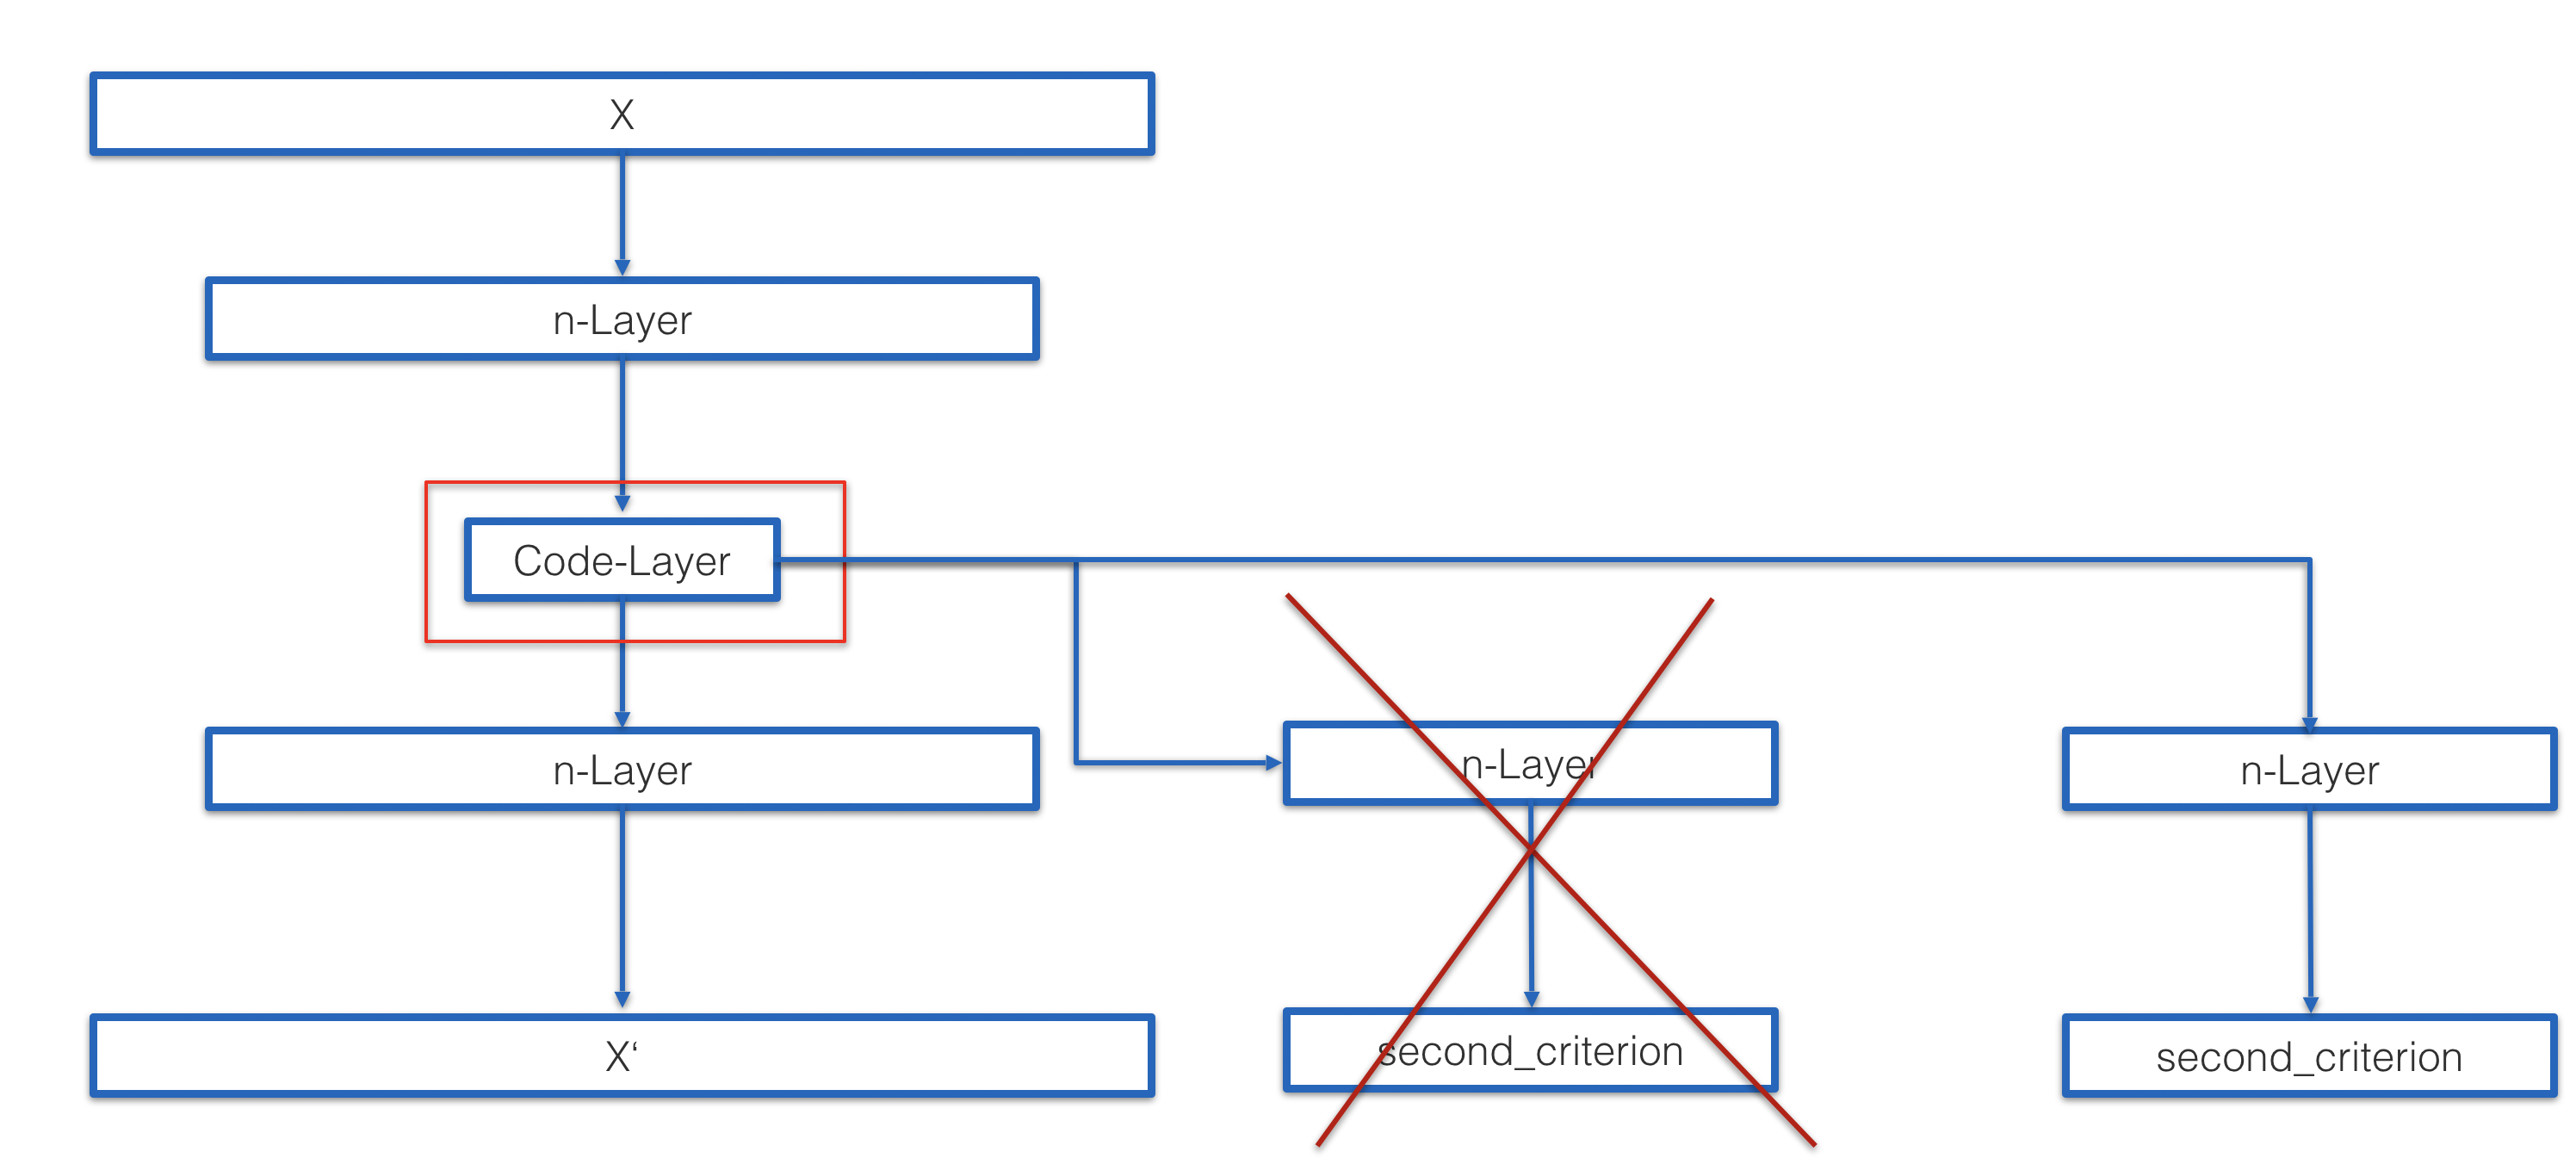
\includegraphics[width=0.5\textwidth, center]{bilder/Schema_Autoencoders/Schema_TSCAE.png}
		\caption[Schema TransferSecondCriterionAutoenocder]{Schema TransferSecondCriterionAutoenocder}
		\label{img:SchemaTSCAE}
	\end{figure}  
	Im Klassendiagramm \ref{img:KlassendiagrammTransferSecondCriterionAutoenocder} für den TSCAE ist zu sehen. Das Besondere ist, dass ein SCAE als Konstruktorargument übergeben wird. Die Einstellungen für den ConvolutionalAutoencoder werden aus diesem Model kopiert. Zusätzlich müssen nur noch die Einstellungen für das zweite Kriterium übergeben werden. Aus diesen wird das Model für das zweite Kriterium erstellt.
	Neu hinzugekommen ist, ein Parameter(freeze\_encoder\_layers) über den eingestellt werden kann, ob und welche Schichten nicht neu trainiert werden können. Es können direkt Schichten ausgewählt werden oder es kann über einen Ganzahlenwert beginnend über die erste Schicht Schichten eingefroren. Werden nur Werte für den Encoder übergeben, werden Werte für den Decoder (freeze\_decoder\_layers) daraus abgeleitet. 
	\begin{figure}[h]
		\centering
		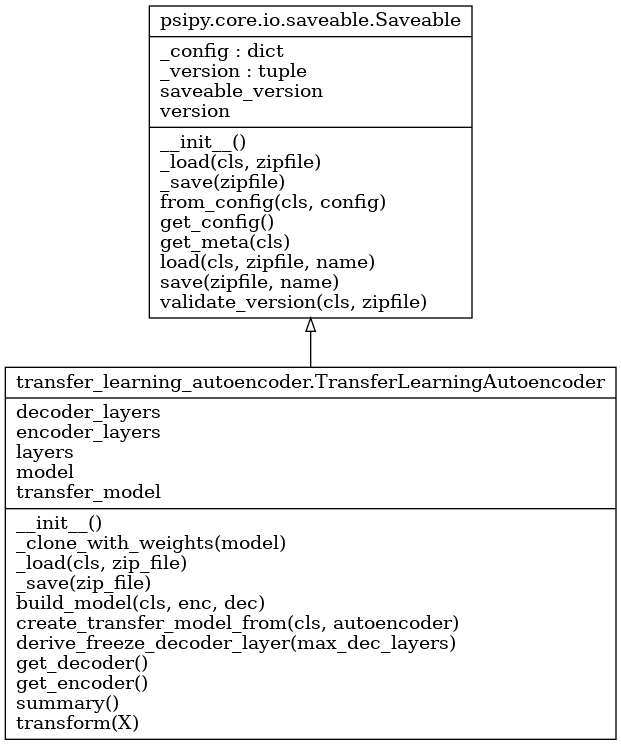
\includegraphics[width=0.5\textwidth, center]{bilder/Klassendiagramme/Klassendiagramm_TLCSCAE.png}
		\caption[Klassendiagramm TransferSecondCriterionAutoenocder]{Klassendiagramm TransferSecondCriterionAutoenocder}
		\label{img:KlassendiagrammTransferSecondCriterionAutoenocder}
	\end{figure}  
	Listing \ref{lst:BspTransferSecondCriterionAutoenocder} zeigt beispielhaft die Anwendung dieses Werkzeuges. Im Vergleich zu dem SCAE ist die Anwendung schon deutlich einfacher. Es gibt weniger Hyperparameter zum Beachten. Da das Modell auf einem trainierten SCAE basiert ist kein $pretrain(..)$ mehr notwenig. Die Methode $fit(..)$ wird auf dieselbe Weiße wie bei SCAE angewendet.	


	\begin{lstlisting}[language=python,caption=Beispiel TransferSecondCriterionAutoenocder in Python, label=lst:BspTransferSecondCriterionAutoenocder]
	tscm = TransferLearningConvolutionalSecondCriterionAutoencoder(csc_autoencoder,
	second_criterion_topology=second_criterion_topology,
	second_criterion_loss = 'binary_crossentropy',                                                                                                   
	second_criterion_hidden_layer_kwargs = {'activation': 'relu'},
	second_criterion_output_layer_kwargs = {'activation': 'sigmoid'}, 
	loss_weights=[1, 0.01],
	freeze_encoder_layers = 2
	,freeze_decoder_layers =[0,1])
	
	history = tscm.fit(
	x_train,
	{"decoder": x_train, "second_criterion": y_train}, 
	epochs=1,
	batch_size = 128,
	validation_data=(x_test,{"decoder": x_test, "second_criterion": y_test}))
	)
	\end{lstlisting}
			
	\section{AutoTransferSecondCriterionAutoenocder}
	\label{sec:AutoTransferSecondCriterionAutoenocder}
	Der AutoTransferSecondCriterionAutoenocder ist ein TransferSecondCriterionAutoenocder welcher mithilfe von HpBandSter AutoML zur Hyperparameteroptimierung einsetzt. Konkret  erbt die Klasse von hpbandster.core.worker. Zur Speicherung und Verwaltung der Hyperparameter wird auf die Klasse HyperparameterMixin zurückgegriffen. Bei der Instanziierung der Klasse werden sinnvolle Standardwerte für Hyperparameter gesetzt. Die Werte können aber später noch angepasst werden. 
	In Abbildung \ref{img:KlassendiagrammAutoTransferSecondCriterionAutoenocder}  ist das zugehörige Klassendiagramm abgebildet. 
	\begin{figure}[h]
		\centering
		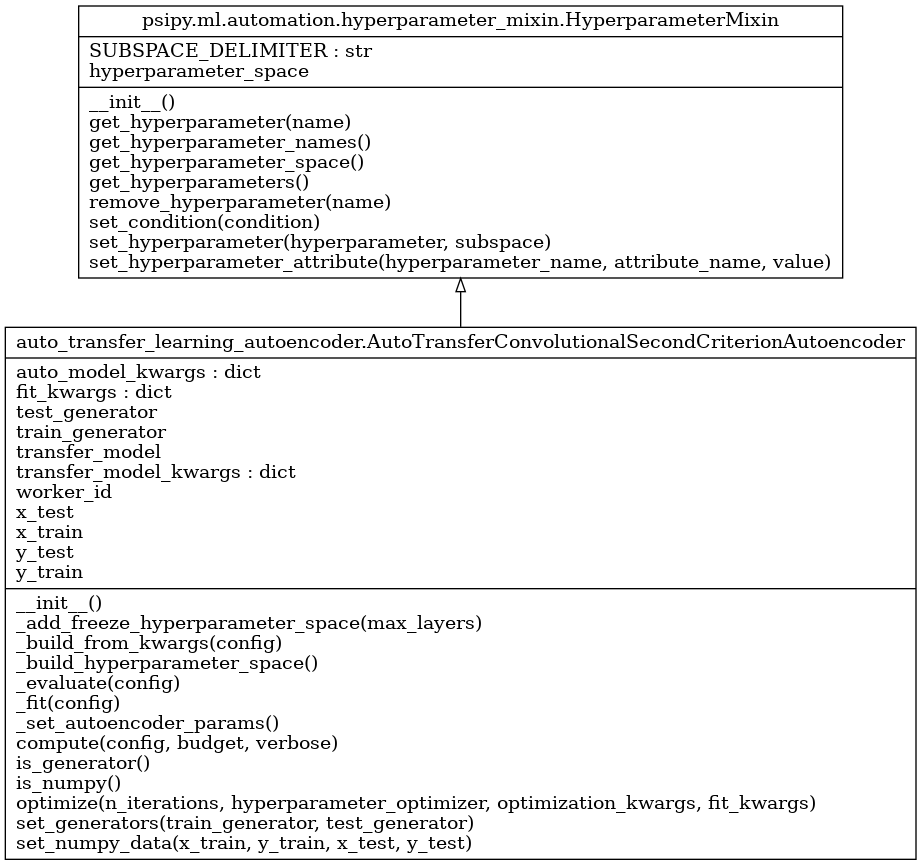
\includegraphics[width=0.5\textwidth, center]{bilder/Klassendiagramme/Klassendiagramm_AutoTLCSCAE.png}
		\caption[Klassendiagramm AutoTransferSecondCriterionAutoenocder]{Klassendiagramm AutoTransferSecondCriterionAutoenocder}
		\label{img:KlassendiagrammAutoTransferSecondCriterionAutoenocder}
	\end{figure}  
	In Listing \ref{lst:BspAutoTransferSecondCriterionAutoenocder} ist eine einfache Implementierung eines AutoTransferSecondCriterionAutoenocder dargestellt. Der Konstruktor unterscheidet sich nur an einer Stelle zum Konstruktor des TransferSecondCriterionAutoenocder. Es wird keine Instanz des SCAE übergeben, sondern ein Pfad zu einem abgespeicherten Modell eines SCAE. 
	Im Gegensatz zur bisherigen Vorgehensweise werden die Trainings und Testdaten mit der Methode $set_generators(..)$  oder $set_numpy_data(..)$ übergeben. Ziel ist es dabei die Komplexität der Methode $optimize(..)$ zu reduzieren. Durch den Aufruf von $optimize(..)$ wird der Optimierungsvorgang gestartet. Die Parameter sind dabei die Anzahl an Iterationen, die Optimierungsstrategie und ein Wörterbuch, welches zusätzliche Einstellungen für die einzelnen Optimierer enthalten kann. In jeder Iteration der Optimierung wird ein neuer TransferSecondCriterionAutoenocder erstellt und mittels der ausgewählten Hyperparameter und übergebenen Daten trainiert. 
	\begin{lstlisting}[language=python,caption=Beispiel AutoTransferSecondCriterionAutoenocder in Python, label=lst:BspAutoTransferSecondCriterionAutoenocder]
	tscm = AutoTransferConvolutionalSecondCriterionAutoencoder(max_deep_freeze=2,
	path_to_model = path_to_base_model,            
	second_criterion_topology=second_criterion_topology,
	second_criterion_loss = 'categorical_crossentropy',                                                                                                   
	second_criterion_hidden_layer_kwargs = {'activation': 'relu'},
	second_criterion_output_layer_kwargs = {'activation': 'softmax'},
	second_criterion_metrics = {'second_criterion':'accuracy'}
	)
	
	tscm.set_generators(train_datagenerator,test_datagenerator)
	
	
	best_config, history = tscm.optimize(3
	,'RandomSearch'
	,optimization_kwargs = optimization_kwargs)
	\end{lstlisting}
	Das Werkzeug unterstützt derzeit die Optimierer, Randomsearch, Hyperband und BOHB.	In Tabelle \ref{table:HyperparparameterAutoML} sind die Hyperaparameter und ihre mögliche Werte dargestellt.
	\begin{table}[ht]
		\centering
		\begin{tabularx}{\textwidth}{lll}
			 \textbf{Hyperparameter} & \textbf{Werte}  & \textbf{Datentyp} 					 	\\
			\textbf{Optimierer}   & 	Adam, sgd, rmsprop		&	Kategorial			\\
			\textbf{Batch\_size}  &  32 - 1024					 &	Ganzzahl			        \\
			\textbf{Epochen}	 &  10 - 10.000				 &	Ganzzahl					 	\\
			\textbf{autoencoder\_loss\_weight}	 	  &  0.01 - 1	 &	Fließkommazahl	\\
			\textbf{second\_criterion\_loss\_weight}	& 0.01 - 1  &	Fließkommazahl	 \\
			\textbf{freeze\_encoder\_layers}	 	  &  0 - Parameter  &	Ganzzahl						\\
			\textbf{freeze\_decoder\_layers}	 	  &  0 - Parameter &	Ganzzahl								
		\end{tabularx}
		\caption{Standard Hyperparameter für AutoML-Suche}
		\label{table:HyperparparameterAutoML}
	\end{table}
	Der Wertebereich für die Stapelgröße wurde aus der Autocrane-Problemstellung abgeleitet. Sie kann maximal, so groß werde, dass kein Speicherplatz-Fehler auftreten kann. Die maximale Anzahl der Epochen wurde bewusst groß gewählt. Es sollen weitere  Problemstellungen ohne viel Konfigurationsaufwand gelöst werden können. Absurd lange Laufzeiten können durch ein EarlyStopping Kriterium verhindert werden. Die Maximalanzahl der möglicherweise einzufrierenden Schichten wird über den Anwender des Werkzeuges definiert, sie sind anwendungsspezifisch.
	
		\todo{weight durch Verhältnis w1/w2 anpassen.}  
	
	\todo{Worker Budget berücksichtingen / notieren}  

	
	